\documentclass[11pt,a4paper]{report}
\usepackage[margin=1in]{geometry}
\usepackage[T1]{fontenc}
\usepackage{lmodern}
\usepackage{hyperref}
\usepackage{booktabs}
\usepackage{longtable}
\usepackage{listings}
\usepackage{xcolor}
\usepackage{tikz}
\usetikzlibrary{shapes,arrows.meta,positioning}

\hypersetup{colorlinks=true,linkcolor=blue,urlcolor=blue}
\lstdefinestyle{bash}{
  basicstyle=\ttfamily\small,
  breaklines=true,
  frame=single,
  backgroundcolor=\color{gray!8}
}

\title{CXR Langfuse Lab Manual\\
\large SW.18 --- LLM traces + full wiring guide}
\author{CXR Ops Lab --- \texttt{cxr-ops-lab}}
\date{2026-05-31}

\begin{document}
\maketitle
\begin{abstract}
\textbf{SW.18}: Langfuse v2 + Postgres on \textbf{:3100}. This manual documents \textbf{exactly how it is wired} ---
Compose $\rightarrow$ UI signup $\rightarrow$ API keys $\rightarrow$ \texttt{send-trace.mjs} $\rightarrow$ Traces tab ---
and where it would attach to Claim Studio judge / doc-reasoning routes in a future phase (not live today).
\end{abstract}
\tableofcontents
\newpage

\chapter{How this lab is wired (step by step)}

\section{The chain (what runs when you type the commands)}

\begin{enumerate}
  \item \textbf{You run} \texttt{./scripts/21-langfuse-up.sh}
  \item Script calls \texttt{docker compose -f compose.langfuse.yaml up -d}
  \item \textbf{compose.langfuse.yaml} starts two containers:
    \begin{itemize}
      \item \texttt{langfuse-postgres} --- Postgres 15, volume \texttt{langfuse\_pg\_data}
      \item \texttt{langfuse} --- image \texttt{langfuse/langfuse:2}, host port \textbf{3100} maps to container \textbf{3000}
    \end{itemize}
  \item \textbf{First browser visit} \texttt{http://localhost:3100} --- sign up (local OSS instance)
  \item \textbf{UI:} \texttt{+ New Organization} $\rightarrow$ create project (e.g.\ \texttt{cxr\_claims})
  \item \textbf{Settings $\rightarrow$ API Keys} --- create keys $\rightarrow$ paste into \texttt{lab/langfuse/keys.env}
  \item \textbf{You run} \texttt{node lab/langfuse/send-trace.mjs} (or \texttt{./scripts/21-langfuse-smoke.sh})
  \item Script loads \texttt{keys.env}, uses Langfuse Node SDK, POSTs trace \texttt{cxr-sw18-golden-path}
  \item \textbf{UI:} Tracing $\rightarrow$ Traces --- golden path appears with mock generation
\end{enumerate}

\section{Wiring diagram}

\begin{center}
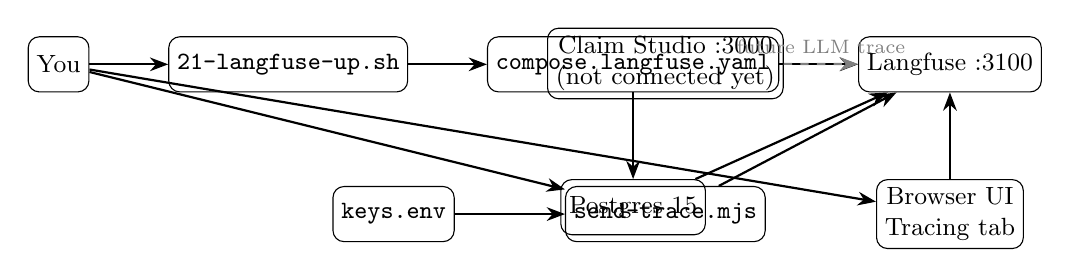
\begin{tikzpicture}[
  node distance=0.55cm and 0.4cm,
  box/.style={draw, rounded corners, minimum height=0.7cm, align=center, font=\small, inner sep=3pt},
  arr/.style={-{Stealth}, thick},
  dashedarr/.style={-{Stealth}, thick, dashed, gray}
]
  \node[box] (you) {You};
  \node[box, right=1cm of you] (up) {\texttt{21-langfuse-up.sh}};
  \node[box, right=1cm of up] (compose) {\texttt{compose.langfuse.yaml}};
  \node[box, right=1cm of compose] (lf) {Langfuse :3100};
  \node[box, below=1.1cm of compose] (pg) {Postgres 15};
  \node[box, below=1.1cm of lf] (ui) {Browser UI\\Tracing tab};
  \node[box, left=1.4cm of ui] (script) {\texttt{send-trace.mjs}};
  \node[box, left=1.4cm of script] (keys) {\texttt{keys.env}};
  \node[box, above=1.1cm of script] (cxr) {Claim Studio :3000\\(not connected yet)};

  \draw[arr] (you) -- (up);
  \draw[arr] (up) -- (compose);
  \draw[arr] (compose) -- (lf);
  \draw[arr] (compose) -- (pg);
  \draw[arr] (pg) -- (lf);
  \draw[arr] (you) -- (ui);
  \draw[arr] (ui) -- (lf);
  \draw[arr] (you) -- (script);
  \draw[arr] (keys) -- (script);
  \draw[arr] (script) -- (lf);
  \draw[dashedarr] (cxr) -- node[above,font=\scriptsize]{future LLM trace} (lf);
\end{tikzpicture}
\end{center}

\chapter{What is wired vs not wired}

\begin{center}
\begin{tabular}{p{4.5cm}p{4cm}p{4.5cm}}
\toprule
\textbf{Layer} & \textbf{Status today} & \textbf{Future (sketch)} \\
\midrule
Langfuse + Postgres :3100 & \checkmark\, Running via Compose & Managed Langfuse Cloud or v3 stack \\
Project API keys & \checkmark\, User-created in UI & CI secret / K8 Secret \\
Golden trace ingest & \checkmark\, \texttt{send-trace.mjs} & Real judge / analyzer spans \\
Claim Studio :3000 & \textbf{Not connected} & \texttt{analyze/route.ts} emits Langfuse spans \\
Rehearsal :8251 & \textbf{Not connected} & OTel + Langfuse dual export \\
Jaeger SW.11 & \textbf{Separate} & Traces vs LLM evals (complementary) \\
\bottomrule
\end{tabular}
\end{center}

\textbf{Today} this lab proves \emph{local LLM observability} and the \emph{golden trace name}
\texttt{cxr-sw18-golden-path} for syllabus M7.8. Claim Studio still runs without Langfuse SDK.

\chapter{Why v2 not v3}

Bootcamp uses \textbf{Langfuse v2 + Postgres only} --- lighter than v3 (ClickHouse, MinIO, Redis, worker).
Port \textbf{3100} avoids collision with CXR Claim Studio on \textbf{:3000}.

\chapter{Golden trace (what \texttt{send-trace.mjs} sends)}

\begin{center}
\begin{tabular}{ll}
\toprule
Field & Value \\
\midrule
Trace name & \texttt{cxr-sw18-golden-path} \\
Input & \texttt{\{ feature: doc-reasoning-sketch, claim\_id: demo-1 \}} \\
Metadata & \texttt{\{ lab: SW.18, syllabus: M7.8 \}} \\
Generation & \texttt{mock-llm-call} / model \texttt{bootcamp-mock} \\
Host default & \texttt{http://127.0.0.1:3100} (override via \texttt{LANGFUSE\_HOST}) \\
\bottomrule
\end{tabular}
\end{center}

\chapter{UI navigation (verified bootcamp path)}

\begin{enumerate}
  \item Open \texttt{http://localhost:3100} --- Home \textbf{Get Started}
  \item \textbf{+ New Organization} (e.g.\ org \texttt{cxr})
  \item Create project (e.g.\ \texttt{cxr\_claims})
  \item \textbf{Settings $\rightarrow$ General} --- confirm host \texttt{http://localhost:3100}
  \item \textbf{Settings $\rightarrow$ API Keys} --- create public + secret key
  \item Copy keys to \texttt{lab/langfuse/keys.env} (\textbf{not} \texttt{keys.env.example})
  \item Run trace script; then \textbf{Tracing $\rightarrow$ Traces} $\rightarrow$ \texttt{cxr-sw18-golden-path}
\end{enumerate}

\chapter{\texttt{keys.env} format (common pitfall)}

The trace script reads \textbf{only} \texttt{lab/langfuse/keys.env}. Lines must be \textbf{uncommented}:

\begin{lstlisting}[style=bash]
LANGFUSE_HOST=http://127.0.0.1:3100
LANGFUSE_PUBLIC_KEY=pk-lf-...
LANGFUSE_SECRET_KEY=sk-lf-...
\end{lstlisting}

\texttt{keys.env} is gitignored. If \texttt{send-trace.mjs} prints \texttt{SKIP}, the file is missing or keys are still commented in \texttt{.example}.

\chapter{Files in the repo}

\begin{longtable}{@{}p{5.2cm}p{7.8cm}@{}}
\toprule
File & Role in the wiring \\
\midrule
\endhead
\texttt{compose.langfuse.yaml} & Postgres + Langfuse v2, port 3100 \\
\texttt{scripts/21-langfuse-up.sh} & Wrapper: \texttt{compose up -d} \\
\texttt{scripts/21-langfuse-smoke.sh} & HTTP :3100 + optional trace ingest \\
\texttt{lab/langfuse/send-trace.mjs} & Langfuse SDK golden trace \\
\texttt{lab/langfuse/keys.env.example} & Template (copy $\rightarrow$ \texttt{keys.env}) \\
\texttt{lab/langfuse/package.json} & \texttt{langfuse} npm dependency \\
\texttt{evidence/SW18-langfuse-verify-2026-05-31.md} & Checklist \\
\bottomrule
\end{longtable}

\chapter{Hypothetical Claim Studio wiring (not deployed)}

\begin{lstlisting}[style=bash]
# Future sketch only:
# 1. npm install langfuse in cxr-ui rehearsal app
# 2. In judge/analyze route: Langfuse client with env from keys
# 3. trace({ name: "cxr-judge", input: claimId, ... })
# 4. generation({ model, prompt, output }) for each LLM call
# 5. Same project keys as bootcamp lab for local dev
\end{lstlisting}

\chapter{Live adjustments}

\begin{itemize}
  \item \textbf{Port 3100} --- deliberate; do not point Langfuse at :3000.
  \item \textbf{v2 image pin} --- \texttt{langfuse/langfuse:2}; v3 needs extra services.
  \item \textbf{First signup} --- data persists in Postgres volume until \texttt{compose down -v}.
  \item \textbf{keys.env vs .example} --- script ignores commented template file.
  \item \textbf{Smoke without keys} --- UI health still passes; trace step SKIPs gracefully.
  \item \textbf{localhost vs 127.0.0.1} --- both work if \texttt{NEXTAUTH\_URL} matches browser URL.
\end{itemize}

\chapter{Procedure}

\begin{lstlisting}[style=bash]
cd cxr-ops-lab
./scripts/21-langfuse-up.sh
# Browser: http://localhost:3100
# Sign up -> org -> project -> Settings -> API Keys
cp lab/langfuse/keys.env.example lab/langfuse/keys.env
# Edit keys.env: uncomment and paste pk/sk
node lab/langfuse/send-trace.mjs
./scripts/21-langfuse-smoke.sh
# Tracing -> Traces -> cxr-sw18-golden-path
\end{lstlisting}

\chapter{Stop}

\begin{lstlisting}[style=bash]
docker compose -f compose.langfuse.yaml down
# Add -v to wipe Postgres (signup + traces)
\end{lstlisting}

\chapter{Bootcamp context}

SW.12--SW.18 electives live in \texttt{cxr-ops-lab} as \textbf{standalone Compose stacks}.
Master port map and cross-lab wiring: \texttt{docs/CXR-BOOTCAMP-LABS-COMPENDIUM.pdf}.

\end{document}
